% !TEX TS-program = Xelatex
% !TEX encoding = UTF-8 Unicode

\documentclass[UTF8]{ctexart}
\usepackage{amsmath}
\usepackage[bottom]{footmisc}
\usepackage{geometry}
\usepackage{graphicx}
\usepackage{hyperref}
\usepackage{figsize}
\usepackage[separate-uncertainty = true,per-mode=symbol]{siunitx}
\usepackage{tabu}
\usepackage{wasysym}
\geometry{left=0.7in,right=0.7in,bottom=0.7in,top=0.7in}
\begin{document}

\title{实验十二:测空气与水中的声速}
\author{朱寅杰 1600017721}
\date{2018年3月9日}
\maketitle
\setcounter{section}{12}
\subsection{今天的声速是多少}
今日风和日丽,天朗气清,实验室的温度计干泡读数为$\theta=\SI{18.7}{\degreeCelsius}$,湿泡读数为\SI{12.5}{\degreeCelsius},得知相对湿度为36\%。实验室有一个水银气压计,读出今日气压为\SI{762.15}{\mmHg}。由此查表计算出,在此温度下,水的饱和蒸汽压为\SI{2.16}{\kPa}。根据书上提供的声速公式(12.8),有
\[
v=\SI{331.45}{\meter\per\second}\times\sqrt{(1+\theta/T_0)(1+0.3192p_w/p)}=\SI{343.0244}{\meter\per\second}
\]
公式中第一项为温度的修正,第二项为湿度的修正。由于后者仅为前者的三十分之一,而温度和湿度的测量精度相近,因此估算不确定度时只需考虑温度修正的不确定度。所用干湿泡温度计的最小分度为\SI{0.5}{\degreeCelsius},故允差取为\SI{0.5}{\degreeCelsius},故$\theta$的不确定度按照均匀分布$1/\sqrt{3}$计,为\SI{.29}{\degreeCelsius},折合入声速的相对不确定度为\num{.0005},相当于\SI{.18}{\meter\per\second}。故声速的计算值可写作$v=\SI{343.0(2)}{\meter\per\second}$
\subsection{驻波共振法测空气中声速}
将超声波发生器的输入频率设置为接近谐振的$f=\SI{38.7}{\kHz}$。保持发生器与接收端基本平行,则可以认为发生器与接收端之间形成一个共振腔;由于声音的波长给定,因此如果腔的长度$l$合适则会形成驻波的振动模式;使用示波器显示接收端声音信号转化出的波形,相邻的观察到极大值出现的位置之间的距离即是声波波长的一半$\lambda/2$,于是测出出现极大值的位置即可得到波长。由于发生器与接收端之间的距离从手轮调节,存在螺纹空程的问题,因此分别记录了$l$增大和减小两个拧手轮方向的数据。见下表(左边是$l$减小组,右边是$l$增大组):
\begin{center}
\begin{tabu}{X[c,-1]|X[c]X[c]|X[c,-1]|X[c]X[c]|X[c,-10]||X[c,-1]|X[c]X[c]|X[c,-1]|X[c]X[c]|X[c,-10]}
\hline
\#	&$l/\si{mm}$	&$U_{pp}$/V	&	\#	&$l/\si{mm}$	&$U_{pp}$/V	&$l_{n+5}-l_n$&\#	&$l/\si{mm}$	&$U_{pp}$/V	&	\#	&$l/\si{mm}$	&$U_{pp}$/V	&$l_{n+5}-l_n$\\
\hline
1	&	58.428	&	0.800	&	6	&	36.215	&	1.12	&22.213	&		10	&	58.534	&	0.820	&	5	&	36.170	&	1.12	&	22.364\\
2	&	53.924	&	0.820	&	7	&	31.770	&	1.18	&22.154	&		9	&	54.113	&	0.860	&	4	&	31.680	&	1.20	&	22.433\\
3	&	49.545	&	0.900	&	8	&	27.418	&	1.36	&22.127	&		8	&	49.607	&	0.900	&	3	&	27.078	&	1.32	&	22.529\\
4	&	45.056	&	0.980	&	9	&	22.770	&	1.56	&22.286	&		7	&	45.242	&	0.960	&	2	&	22.746	&	1.56	&	22.496\\
5	&	40.418	&	1.04	&	10	&	18.542	&	1.74	&21.966	&		6	&	40.545	&	1.02	&	1	&	18.542	&	1.74	&	22.003\\
\hline
\end{tabu}
\end{center}
对测得的$l$按照$l_{n+5}-l_n$进行逐差(见表中),并取平均计算出半波长$\lambda/2$的测量值,从两组数据里算出的分别为\SI{4.46984}{\mm}与\SI{4.473}{\mm}。根据数据的方差估计出其对这两个半波长计算值的不确定度分别为\SI{0.0455}{\mm}与\SI{0.0190}{\mm}。读数手轮一格是\SI{.01}{\mm},按照\SI{.005}{\mm}取允差,得到仪器不确定度对半波长的不确定度的贡献约为\SI{.0006}{\mm}。分别合成进去,得到半波长的测量值为\SI{4.47(5)}{\mm}与\SI{4.47(2)}{\mm},乘以上面的发生器频率(不确定度与之相比可以忽略)得到声速测量值为\SI{346(4)}{\meter\per\second}与\SI{346(2)}{\meter\per\second}。

\begin{figure}
  \centering
  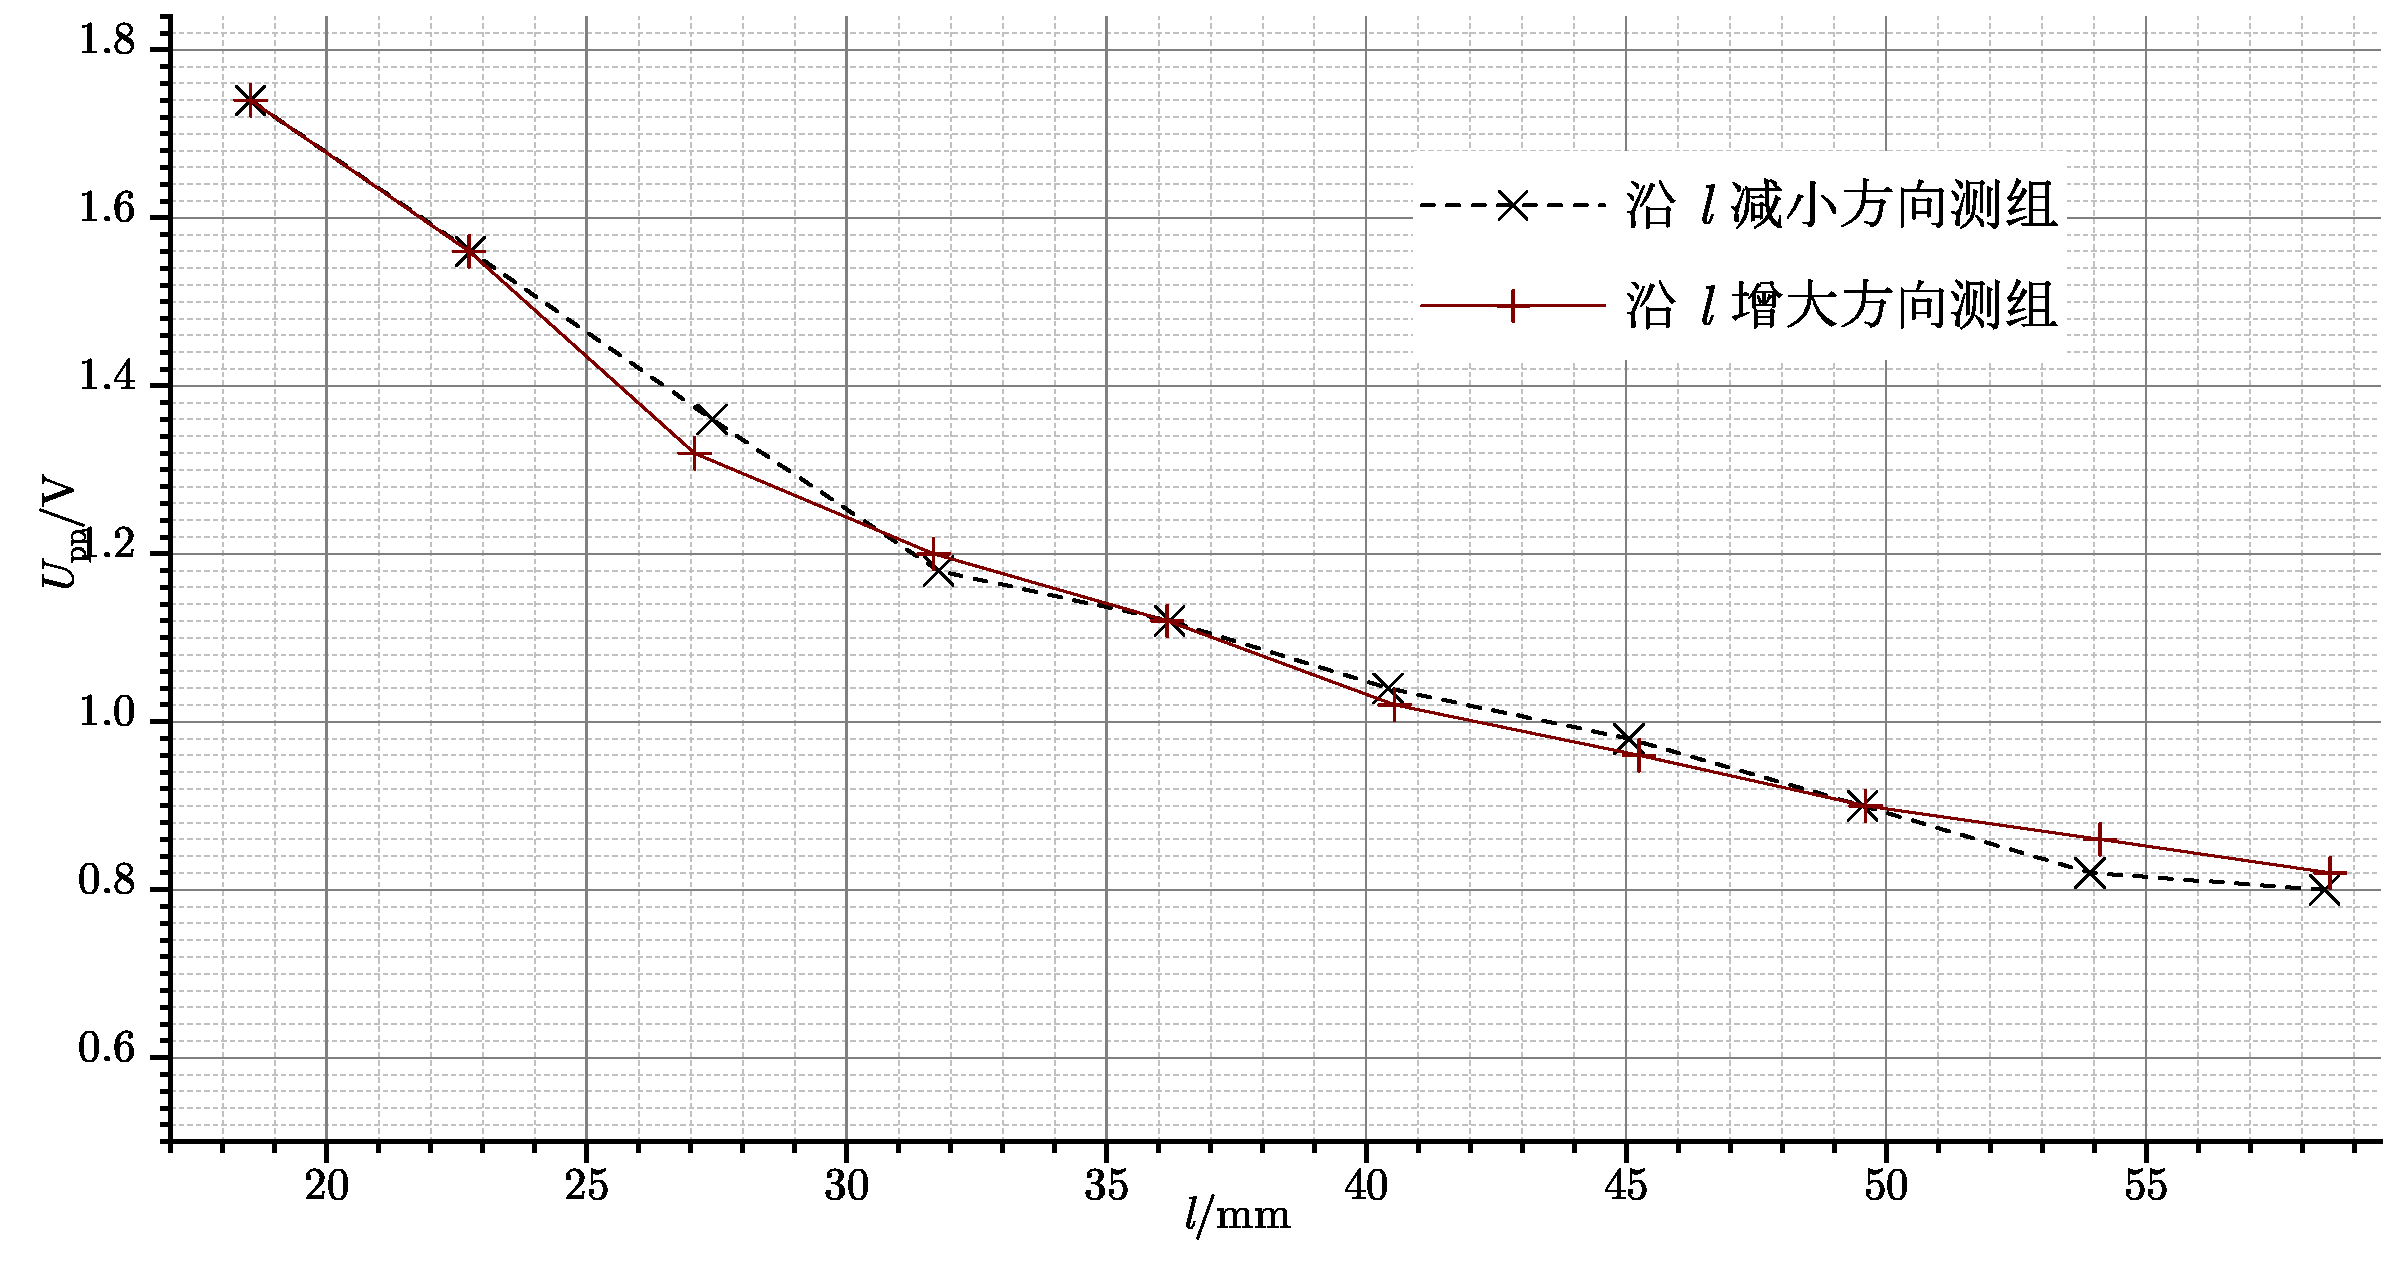
\includegraphics[width=\linewidth]{Upp.eps}
  \caption{图示两组测量得到的各个极大位置处接收器电平振幅,可从中观察声波随距离衰减的特征。}
\end{figure}


\subsection{行波相位法测空气中声速}
同样将超声波发生器的频率设置为$f=\SI{38.7}{\kHz}$,将发生端与接收器两路信号同时接入示波器以$X-Y$模式显示。两路信号应该频率相同,相差一个相位(即是声波传播造成的相位差),因此能观察到利萨如图形。发生端与接收器的距离每改变一个波长,两路信号的相位差变化$2\pi$,因此记录下每处利萨如图形拉成正直线的位置,即可得到波长。仍然和上面一样,测量一去一回。
\begin{center}
\begin{tabu}{X[c]X[c]X[c]X[c]X[c]X[c]X[c]X[c]X[c]X[c]X[c]}
\hline
$l$/mm	&1&2&3&4&5&6&7&8&9&10
\\
\hline
移近&104.301 	&95.382 	&86.411 	&77.449 	&68.585 	&59.648 	&50.972 	&41.869 	&33.118 	&23.985 \\
移远&104.202 	&95.343 	&86.382 	&77.420 	&68.570 	&59.654 	&50.988 	&41.900 	&33.174 	&24.052 \\
\hline
\end{tabu}
\end{center}
用学校买的Origin对数据进行最小二乘拟合。不计允差,移近一组的数据软件计算得到斜率(亦即波长的估计值)为\SI{8.9077(103)}{\mm},移远一组的数据软件计算得波长的估计值为\SI{8.89185(1034)}{\mm},两个相关系数均在五个九以上。\footnote{Origin对斜率的不确定度的计算方法参阅\url{https://www.originlab.com/doc/Origin-Help/LR-Algorithm\#Fit_Parameters},算法是与书上公式一致的。}再合成入各位置测量值的允差:如同上面一样,允差造成的位置测量不确定度大概是\SI{.0029}{\mm},按照书上公式(7.17),除以自变量(也就是1到10的指标)的标准差的十倍(约是\num{9.083}),得到对波长不确定度的贡献约为\SI{.0003}{\mm}。将这一值按方和根合成入上面两个不确定度(实际上由于大小相差悬殊合成进去并无影响),得到波长分别为\SI{8.91(1)}{\mm}与\SI{8.89(1)}{\mm},乘上频率得到声速测量值分别为\SI{344.7(4)}{\meter\per\second}与\SI{344.1(4)}{\meter\per\second}。
\subsection{利用超声光栅衍射测水中声速}
使用频率已知的发生器在水中产生一个超声波信号,纵波产生周期性的疏密结构,形成一个不事雕琢的天然光栅,光栅的周期即是声波的波长。因而利用衍射确定光栅周期即可测出水中声速。实验时发生器的频率为\SI{9.650}{\MHz},使用波长为$\lambda=\SI{632.8}{\nm}$的氦氖红光进行衍射,在距离衍射面$L=\SI{752}{\cm}$(使用卷尺测出)的墙面上观察衍射花样。使用刻度尺量出相邻两级条纹之间距离$d$分别为\SI{3.02}{\cm}、\SI{3.05}{\cm}、\SI{3.08}{\cm}、\SI{3.04}{\cm}、\SI{3.15}{\cm}、\SI{3.05}{\cm}、\SI{3.07}{\cm}、\SI{3.12}{\cm},平均为\SI{3.073}{\cm}。根据公式得到光栅周期为$L\lambda/d=\SI{154.9}{\micro\meter}$,从而有水中声速为\SI{1494.6}{\meter\per\second}。考虑卷尺和钢刻度尺的不确定度,结果的不确定度大概在百分之一左右。
\subsection{讨论}
测量多个极大位置做逐差或是最小二乘拟合,得到结果的不确定度当然比只测两个极大位置好得多啦。李萨如法还好些,那个共振法看振幅极大,不管是凭肉眼观察还是凭示波器指示,都难以确定一个准确的位置,因此实际上上面计算允差只考虑手轮读数的误差实在是大大低估了;好在这一读数的困难在随机误差里部分地得到了体现。如果不逐差只是简单取平均的话,相当于浪费了中间测量的数据点,并不可取。正弦波振幅极大总是比极小容易判断一些(虽然也并不好判断),李萨如图线也是,直线位置比其他位置在定位的精确度上高得多。

声波信号随距离衰减,应该是服从类似平方反比的规律的,大致就是长上面画的那幅图那个样。

这个实验也是从小做到大了,驻波法、行波法和多普勒法在高中做过好多遍,也是观感最亲切的实验之一。然而还是常做常新的,一方面以前没做过超声光栅法(只是听人说起过),另一方面这次实验用的示波器是实验经历里用过最智能最高级的,甚至能够自动调节,并且把信号存储到U盘里,体验挺不错。
\end{document} 